
%(BEGIN_QUESTION)
% Copyright 2008, Tony R. Kuphaldt, released under the Creative Commons Attribution License (v 1.0)
% This means you may do almost anything with this work of mine, so long as you give me proper credit

Examine this process trend, showing the response of the process variable to a 10\% up-and-down step change in the controller output (placed in manual mode):

$$\includegraphics[width=15.5cm]{i03483x01.eps}$$

Based on this open loop response, qualitatively predict the necessary P, I, and D actions of the controller, using terms such as ``none,'' ``weak,'' ``moderate,'' and ``aggressive.''

\vskip 10pt

Proportional = \underbar{\hskip 70pt} \hskip 20pt Integral = \underbar{\hskip 70pt} \hskip 20pt Derivative = \underbar{\hskip 70pt}

\vskip 10pt

Also determine whether the controller needs to be {\it direct-acting} or {\it reverse-acting}.

\underbar{file i03483}
%(END_QUESTION)





%(BEGIN_ANSWER)

3 points for P, 2 points each for I and D, 3 points for action.

\vskip 10pt

\noindent
Proportional = \underbar{{\bf Aggressive} or {\bf Moderate}} \hskip 10pt Integral = \underbar{{\bf None} or {\bf Weak}} \hskip 10pt Derivative = \underbar{{\bf None} or {\bf Weak}}

\vskip 10pt

The controller needs to be {\bf reverse-acting}.

%(END_ANSWER)





%(BEGIN_NOTES)

{\bf This question is intended for exams only and not worksheets!}.

%(END_NOTES)


